\chapter{}

\begin{figure}
\centering
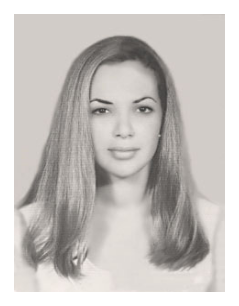
\includegraphics[width=0.7\linewidth]{16/carteira-de-trabalho.png}
\caption{Foto da minha primeira carteira de trabalho.}
\end{figure}

Aos vinte e um anos, obediente às recomendações da minha mãe, mesmo não sendo bonita eu \textbf{\textit{parecia}} sê-lo, após anos de aprendizado de como devia vestir-se, pentear-se, maquilar-se e comportar-se uma moça em sociedade.
Porque tal como predissera minha mãe, muito acertadamente, a convivência com as abonadas pupilas das cônegas agostinianas constituíra-se numa verdadeira escola de bom gosto e sofisticação.
Aprendizado reforçado pela assessoria da Tia Maria Angelina e das amigas de pensionato.
Os cabelos, agora longos, clareados e bem tratados, emolduravam um rosto mais harmônico, onde se destacava o nariz esculpido pelas hábeis mãos do Dr.
Fabrini, um renomado cirurgião plástico carioca.
Magra, ou pelo menos tão magra como jamais voltaria a ser, eu começava a achar divertida a situação de provocar admiração no público masculino.
Pela aferição das ruas, baseada em observações tão cruas quanto espontâneas de motoristas, pedreiros e \textit{office-boys}, eu me incluía entre as chamadas “boazudas”: alta, pernas grossas, quadris roliços e cintura fina.
A situação me era totalmente inusitada: provocar olhares à minha passagem, ser confundida com estrelinha de televisão, ver-me notada e seguida por rapazes, era uma novidade sem precedentes na minha vida.
Por sorte, paralelamente, havia trabalhado duro para superar minha timidez, melhorar minha capacidade de comunicação e conseguia com relativa facilidade impor-me frente à maioria das situações.
Em nenhum momento inebriei-me com essa admiração que eu, mais do que ninguém, sabia que resultava de pura ilusão ótica.
Não sou bonita, nunca fui, mas estava segura de produzir o efeito que uma vez um velho fazendeiro creditou à tia Odila: sem saber como definir o bem-estar que a sempre afirmativa presença dela lhe provocava, saiu-se com esta: “- Dona Odila, dá gosto ver a senhora assim, sempre tão \textbf{saudível e calorífera}!”.
É isso, tinha certeza de não ser bonita, mas desde a minha mocidade e até hoje, venho me empenhando em produzir a impressão de uma personalidade “saudível e calorífera”.
É o que pessoalmente designo como dever ecológico, isto é, a obrigação de contribuir para tornar o mundo um lugar mais agradável, exibindo uma aparência que tem menos a ver com elegância ou beleza e mais com certo jeito de ser.
No entanto, a descoberta de que podia exercer algum poder sobre o gênero superficial e tolo dos garanhões de plantão, tenho que admitir, encantou-me durante algum tempo e me manteve a salvo de interessar-me verdadeiramente por alguém.
Claro que para isso concorria também o fato de me conservar firme na disposição de jamais me casar.
Foi por essa altura que apareceu Paulo.

O ano que sucedeu à minha formatura, 1969, foi marcado pela derrubada de mais algumas fantasias que eu alimentava a meu próprio respeito.
Eu não queria voltar para Araraquara e procurava ansiosamente uma maneira de permanecer na Capital às minhas próprias custas.
Sabia que andava exigindo do meu pai mais do que era justo pretender.
Eu era a mais velha de cinco, já tinha passado da hora de saltar do berço.
Porém, sustentar-me com o salário de professora, em São Paulo só seria possível se eu tivesse coragem e iniciativa para aceitar trabalho onde aparecesse, o que podia significar tomar ônibus de manhã cedinho e voltar à noite, depois de enfrentar colégios públicos de periferia e renunciar às roupinhas, sapatinhos de moda e mais alguns adereços importantes para o meu recém-adquirido \textit{status} de beldade.
Na verdade, eu avançara muito pouco na direção da tão sonhada autonomia.
Na essência, continuava a mesma burguesinha assombrada por receios provincianos de enfrentar a selva da cidade grande e, mais do que isso, de viver por minha própria conta e risco, sem depender da mesada do papai.


Entrementes o governo, depois de longo tempo, decidiu promover em meados do ano um concurso para prover cargos de professores nas escolas públicas de todo o Estado de São Paulo.
Era a deixa que meu pai esperava para por fim à minha interminável, infrutífera e onerosa permanência em São Paulo.
Conformada, inscrevi-me, com a esperança de que até o concurso algum emprego aparecesse.
Estávamos em janeiro, ainda.

Um dia, andando pela faculdade, reencontrei Regina Pereira, minha antiga, esgalgada e neurótica companheira de quarto no pensionato.
Esfuziante, participou-me seu casamento no sábado seguinte e exigiu que eu me incluísse na comitiva de ex-colegas que se preparava para comparecer ao casório, em Poços de Caldas.
Fui.
No meio da festa, um rapaz sentou-se ao meu lado e não me largou mais.
Alto e magro, moreno como um árabe, olhos muito escuros, calado, não parecia nem um pouco divertido.
Ao contrário, era um tanto brusco e logo descobri que minhas táticas habituais de lidar com esse tipo de situação não funcionavam com ele.
Em pouco tempo desconstruiu todas e como costumava acontecer comigo quando me via desarmada e insegura, chorei.
Só então ele pareceu abrandar e decidiu ser gentil.
Comprou-me chocolates.
Ao voltar para São Paulo, estava decidida a esquecê-lo.
Ele me figurava uma ameaça.
Chamava-se Paulo e era um ex-namorado da noiva.
 
Dias depois, no Carnaval, fui para Araraquara porque participava de um bloco que desfilava no Clube todos os anos.
Estava eu lá, dançando na maior animação, quando uma amiga veio me avisar, um tanto preocupada, que um rapaz estava à minha espera no saguão.
A preocupação se justificava pelo fato de que minha família estava presente e meu pai, cujo gênio todos conheciam, já parecia sensivelmente alterado pelo uísque.
 Instintivamente, soube que era o Paulo.
Corri escada abaixo, disposta a despachá-lo para longe, evitando um previsível confronto.
Papai, desde alguns anos, vinha se convertendo num problema para todos nós.
Nunca soubemos se de alguma maneira pressentia a iminente doença cardíaca que o levaria ao túmulo, depois de limitar-lhe drasticamente a vida, ou se a aproximação da velhice e da decadência física lhe parecia intolerável porque mamãe, bem mais nova, estava no auge da sua disposição para a vida.
O fato é que papai vinha abusando sistematicamente da bebida e com isso se transformou numa versão particular de Dr.
JekiIl e Mr. Hyde: de dia, um homem equilibrado, sensato e bonachão; à noite, sob o efeito do álcool, um sujeito violento e imprevisível, capaz de atitudes de extrema agressividade e de completa falta de consideração por quem quer que fosse.
Como costuma acontecer nessas circunstâncias, evitávamos ao máximo levar amigos ou namorados em casa, eu mais do que os outros.
Mas, Paulo não era homem de se assustar com isso.
Eu ainda não sabia que, em matéria de loucura familiar, ele já conhecia tudo.
Não arredou pé e eu tremi sob os olhares arrevesados que meu pai lançava a intervalos sobre nós dois.
Consegui que Paulo concordasse em me levar para casa para afastá-lo dali, mas ainda nos despedíamos diante da porta quando o carro do meu pai virou a esquina acelerado, passou chispando por nós e invadiu a garagem sem reduzir a marcha.
Freou, guinchando, a centímetros da parede.
Gelada, ouvi, às minhas costas os argumentos desesperados da minha mãe, tentando fazer um alterado Mathias entrar sem dar vexame.
 Minha irmã, que chegara com eles no carro, através da janela entreaberta do nosso quarto, fazia sinais aflitos para eu entrar.
Finalmente, para meu alívio, Paulo decidiu ir embora.
Pulando a janela para não passar pela porta do quarto dos meus pais, onde a discussão prosseguia acalorada, estendi-me como um cadáver na cama, envolta na túnica, nas pulseiras e colares da minha fantasia tribal africana.
Acordei, na manhã seguinte, com minha mãe assustada pedindo que eu me levantasse e me arrumasse, porque “aquele moço” estava na varanda conversando com meu pai e, pelo que ela tinha entendido, os dois estavam saindo para ir ao clube tomar umas cervejas e conversar.
 Foi assim que Paulo entrou na minha vida para nunca mais sair.

\begin{figure}
\centering
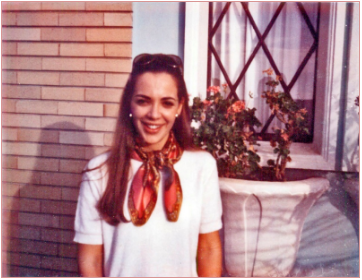
\includegraphics[width=0.7\linewidth]{16/eu-quando-paulo.png}
\caption{Eu, em 1969, quando conheci Paulo.}
\end{figure}

Ao longo das periódicas crises que o evoluir de um casamento propõe à gente, muitas vezes me perguntei se cheguei ao casamento por vontade própria ou se me deixei vencer pela tenacidade indomável do Paulo e pela capacidade extraordinária que ele tinha de reduzir a pó todo o meu tão bem arrumadinho sistema de defesa.
A verdade é que, com seu temperamento, ele expunha toda a frágil arquitetura da minha personalidade, tão cuidadosamente edificada ao longo dos anos para encobrir minhas inseguranças.
Eu levaria um longo tempo para entender que o que me punha em cheque era a exigência de verdade, de autenticidade que nele é permanente e intransigente.
Os traumas decorrentes da sua história familiar provocavam nele reações surpreendentes de intolerância a qualquer forma de manipulação ou jogo, por inocente que fosse.
Acostumei-me a compará-lo a um animal mal domesticado, cujo instinto alerta para a condição de ter no homem um inimigo natural e que, por uma folha que se agita, pode atirar-se sobre o dono, atacando-o.
Custei muito a aprender a lidar com esse jeito dele e a sensação constante de estar indefesa resultou na desconfiança de ter me tornado, eu sim, manipulável.

Hoje, passados muitos anos, inclino-me a concluir que ambos fomos envolvidos numa espécie de irresistível conspiração cósmica.
De outra maneira, como poderiam ter se juntado duas criaturas tão pouco propensas a acreditar em quem quer que fosse?
